\documentclass{article}
\usepackage{xyreport}
\makeatletter
\def\maketitle{%
%  \thispagestyle{empty}%这部分是另标题单独占一页
%  \vfill
  \begin{center}%\leavevmode
    \vspace{1em}
    \normalfont
    {\sanhao \bf \@title\par}%
    \vspace{2em}   %缩小题目和作者名字之间的行距,这里是1毫米
    {\xiaosi \@author\par}%
    \vspace{2em}
    {\xiaosi \@date\par}%去掉%显示日期
    \vspace{3em}
    \vspace{1em}
  \end{center}%
%  \vfill
%  \cleardoublepage  %结束当前页,下一页从奇数页开始
  }
\makeatother
\graphicspath{{figures/}}
\title{光线跟踪实验报告}
\date{2014年1月6日}
\author{基科11 刘心宇 2011012135}
\begin{document}
\maketitle
\tableofcontents
\newpage
\section{实验目的}
用C++实现光线跟踪算法。
\section{实验内容}
\begin{compactitem}
\item 三维场景的描述
\item 基本光线跟踪算法(Ray Tracing)
\item 软阴影(Soft Shadow)
\item 纹理(Texture)
\item 景深(Depth Of Field)
\item 空间加速(BSP Tree)
\end{compactitem}
\section{实验原理}
\subsection{三维场景描述}
可以用参数化的方法描述最基本的几何体包括平面,球体和立方体等。对于复杂的三维物体,可以用专业的建模软件建模,生成obj文件,并导入。
\subsection{基本光线跟踪算法(Ray Tracing)}
我们之所以能看到物体,是应为光线从光源出发经过一系列的反射折射最终进入视点。光线跟踪算法采用逆向的方法,假设光线从试点出发,投射在场景中,计算颜色,并对反射和折射光线继续进行跟踪,将所得颜色按照系数与当前颜色叠加,最终完成绘制,是一种递归算法。虽然在理想情况下,光线可以在物体之间进行无限次的反射和折射,但在实际算法中,当光线的强度小于最小阈值或者没有与物体相交时,终止递归。光线跟踪算法可以实现其它算法来很难达到的效果,它作为一个有效的真实感图形绘制算法被广泛地使用。\cite{graphics} 光线跟踪伪代码如下:
\renewcommand{\lstlistingname}{Algorithm}
\begin{lstlisting}[caption=RayTracing]
RayTracing (start, direction, weight, color)
{
    if (weight < MinWeight)
        color = black
    else
    {
        计算光线与所有物体交点中距离 start 最近的点 P;
        if ( 没有交点 )
            color = black;
        else
        {
            Ilocal = 在交点处采用局部光照模型计算出的光强;
            计算反射光线的方向 R;
            Raytracing (P, R, weight*wr, Ir);
            计算反射光线的方向 T;
            Raytracing (P, T, weight*wt, It);
            color = Ilocal + Ir + It;
        }
    }
}
\end{lstlisting}\ecode
\subsubsection{Phong模型}
在计算交点处的局部光照时,采用Phong模型。Phong光照模型可以表述为:由物体表面上一点P反射到视点的光强$I$为环境光的光强$I_e$、理想漫反射光强$I_d$和镜面反射光$I_s$的总和,即$$I=I_aK_a+I_pK_d(L\cdot N)+I_pKs(R\cdot V)^n$$其中$K_d$为漫反射系数,$K_s$为镜面反射系数。图\ref{fig:phong}显示了Phong模型中的几何量。
\begin{figure}[H]
\centering
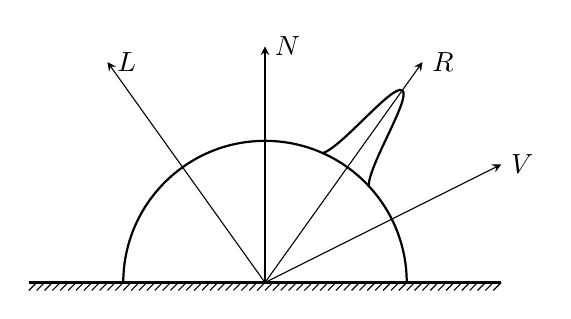
\begin{tikzpicture}
\draw[thick] (0:0) -- (0:1.8) arc (0:180:1.8) -- (0:0) -- cycle;
\draw[thick] (0:-3) -- (0:3);
\draw[->,>=stealth] (0,0) -- (2,2.8) node[right] {$R$};
\draw[->,>=stealth] (0,0) -- (-2,2.8) node[right] {$L$};
\draw[->,>=stealth] (0,0) -- (0,3) node[right] {$N$};
\draw[->,>=stealth] (0,0) -- (3,1.5) node[right] {$V$};
\draw[thick] (0.7344,1.6434) .. controls (0.9942,1.7354) and (1.6195,2.5253).. (1.7437,2.4412);
\draw[thick] (1.3164,1.2277) .. controls (1.3191,1.5033) and (1.8635,2.3510).. (1.7437,2.4412);
\foreach \i in {-2.9,-2.8,...,3}
{
  \draw (\i,0) -- (\i-0.1,-0.1);
}
\end{tikzpicture}
\caption{Phong模型中的几何量}
\label{fig:phong}
\end{figure}
\subsubsection{光线求交}
针对不同的几何体,有不同的求交算法,在此不在赘述。
\subsubsection{阴影}\label{sec:shadow}
在计算局部光照模型时,判断图\ref{fig:phong}中交点和光源的连线$L$是否与其他物体相交,如果相交,则该交点处在阴影区,否则不是。处在阴影区的点局部光强就是环境光,无漫反射和高光。
\subsection{软阴影(Soft Shadow)}\label{sec:softshadow}
理想点光源,每一个交点只有是阴影和不是阴影两种状态,所以在阴影的边缘十分明显。但现实情况并非如此,为了实现软阴影的效果,可以将面光源看成若干个点光源,然后加权平均,所得到的阴影边缘会有渐变,更加真实。
\subsection{纹理(Texture)}
需要将物体表面的坐标和位图的坐标对应起来,也就是纹理坐标。由于选择的几何体都是参数化的描述,所以很容易建立纹理坐标,实现纹理映射。
\subsection{反锯齿(Anti-aliasing)}
消除物体边缘的锯齿效果,本次实验中采用最简单但并不高效的方法,用4倍采样,相当于高分辨率的图像缩小,会有效地减少锯齿。
\subsection{景深(Depth Of Field)} 
景深是指相机对焦点前后相对清晰的成像范围。虽然透镜只能够将光聚到某一固定的距离,远离此点则会逐渐模糊,但是在某一段特定的距离内,影像模糊的程度是肉眼无法察觉的,这段距离称之为景深。\par
现实中景深通常由物距、镜头焦距,以及镜头的光圈值所决定。且焦平面前后的景深距离也并不相同。为了实现方便,我们假设景深与物距无关,且前后相同,因此用两个参数描述景深,焦距和光圈大小。\par
具体实现时,在做光线跟踪的同时,记录每一个像素的深度值(深度缓存)。然后用每一个像素的到焦平面的距离作为参数和光圈大小,做模糊处理。这个方法是基于深度缓存的后期处理,并不是对于透镜的模拟(可以用分布式光线跟踪算法),所以得到的效果可能并不那么真实,是一种近似处理。
\subsection{空间加速(BSP Tree)}
BSP 树是一种二叉树,用于加速光线与大量物体求交的过程。在树中每个叶
节点上维护一个链表,存储该节点上的所有物体;同时在每个节点上存储一个
AABox(axel-aligned box),表示该节点对应的空间区域。初始时树中只有根节
点,且其上的链表为空,AABox 为整棵树所对应的子空间。
\begin{itemize}
\item \textbf{插入物体} 物体被插入到所有满足以下条件的叶节点中:从根到该叶节点的
路径上的每个节点的AABox 均与该物体相交。物体被插入一个叶节点时,
如果该节点深度小于一个预设常数且该节点上已有的物体个数达到某预设
常数时,先对节点进行分割再接着在子树上插入。
\item \textbf{分割叶节点} 当某叶节点U上的物体个数达到某常数,且节点的深度未达
某常数时,则需要对叶节点进行分割。分割方法为:为U 分配两个子节
点$V_1,V_2$,将U的AABox 沿着最长边等分成两个小的AABox 并分别赋
给$V_1,V_2$;再使用上述插入算法,将U上原有的每个物体插入到以U为根
的子树上,并清空U上的物体链表。
\item \textbf{光线求交} 如果U 是叶节点,则遍历U 上的所有物体分别求出交点,其中
距光源最近且在U 的AABox 内部的交点即为所求交点。\\
否则,先求出光线与U 的两个子树$V1,V2 $的AABox 的交点,不妨设与$V_1$
交点的距离严格小于与$V_2$交点的距离(如果不相交,则认为距离是无穷远),
或者两者距离相等但光源在$V_1$内部。此时,先递归求解光线与$V_1$子树中
的物体的最近交点,如果有交点则为最终所求交点;否则再递归求解光线
是否与$V_2$子树中的物体有交点。\\
需要特别注意的是,如果光线与$V_1,V_2$的AABox 交点到光源距离相等但光
源不在任何一个的内部,则应递归与两者上的物体都求交,再取最近者。
\end{itemize}
\vspace{0.5em}
\section{编程实现——文件结构和类设计}
\begin{tabbing}
\hspace*{2em}\=文件\hspace*{8em} \=说明\hspace*{20em}\kill
\>.$\backslash$XY.h\>全局函数定义,宏定义\\
\>.$\backslash$XYClass.h\>所以类型定义\\
\>.$\backslash$BSPTree.cpp\>AABox和BSPTree类,实现空间加速\\
\>.$\backslash$XYCamera.cpp\>XYCamera类,实现渲染,其中包含光线跟踪算法\\
\>.$\backslash$XYLight.cpp\>XYLight和XYLightSource类,描述灯光\\
\>.$\backslash$XYMath.cpp\>XYVector3类,实现向量运算\\
\>.$\backslash$XYObject.cpp\>简单几何体,基类XYObject,派生类XYPlane,XYShpere,XYTriangle,XYBox\\
\>.$\backslash$XYScene.cpp\>XYScene类,描述场景,物体的集合,处理求交,使用BSPTree加速\\
\>.$\backslash$XYTexture.cpp\>XYTexture类,描述纹理\\
\>.$\backslash$XYTime.cpp\>计时模块\\
\>.$\backslash$XY.cpp\>其他辅助类,全局函数实现\\
\>.$\backslash$main.cpp\>测试用例\\\\
\>//网格模型解析(助教提供)\\
\>.$\backslash$SimpleObject.h\>\\
\>.$\backslash$Vec3f.h\>\\
\>.$\backslash$SimpleObject.cpp\>\\
\>.$\backslash$Vec3f.cpp\>
\end{tabbing}
\section{效果演示}
\subsection{Phong模型} 
图~\ref{fig:phongdemo}中展示了Phong模型示例,即局部光照=环境光+漫反射+高光
\begin{figure}[H]
  \centering%
  \subfloat[环境光]{
    \label{subfig:p1}
    \includegraphics[width=0.22\textwidth]{0.jpg}}
  \subfloat[漫反射]{
    \label{subfig:p2}
    \includegraphics[width=0.22\textwidth]{1.jpg}}
  \subfloat[高光]{
    \label{subfig:p3}
    \includegraphics[width=0.22\textwidth]{2.jpg}}
  \subfloat[叠加]{
    \label{subfig:p4}
    \includegraphics[width=0.22\textwidth]{3.jpg}}
  \caption{Phong模型示例}
  \label{fig:phongdemo}
\end{figure}
\subsection{反射与折射}
运用光线跟踪算法求解全局光照,可以得到反射折射的效果,如图~\ref{fig:rr}所示。
\begin{figure}[H]
  \centering%
  \subfloat[反射]{
    \includegraphics[width=0.3\textwidth]{5.jpg}}
  \subfloat[折射]{
    \includegraphics[width=0.3\textwidth]{4.jpg}}
  \caption{反射与折射}
  \label{fig:rr}
\end{figure}
\par
考虑可能会出现全反射的情况,如图~\ref{fig:tir}所示。更多效果请见附件tir.mp4。
\begin{figure}[H]
  \centering%
    \includegraphics[width=0.3\textwidth]{18.jpg}
    \includegraphics[width=0.3\textwidth]{19.jpg}
  \caption{反射与全反射}
  \label{fig:tir}
\end{figure}
\subsection{阴影与软阴影} 
在求解全局光照时,增加一次求交运算(见\ref{sec:shadow}),可以得到阴影效果。将面光源看成若干个点光源的集合(见\ref{sec:softshadow}),就可以产生软阴影的效果,如图~\ref{fig:shadow}所示。
\begin{figure}[H]
  \centering%
  \subfloat[硬阴影]{
    \includegraphics[width=0.3\textwidth]{7.jpg}}
  \subfloat[软阴影]{
    \includegraphics[width=0.3\textwidth]{6.jpg}}
  \caption{阴影与软阴影}
  \label{fig:shadow}
\end{figure}
\subsection{反锯齿}
4倍采样,得到反锯齿的效果,如图~\ref{fig:aa}所示。
\begin{figure}[H]
  \centering%
  \subfloat[1倍采样]{
    \includegraphics[width=0.35\textwidth]{9.jpg}}
  \subfloat[4倍采样(反锯齿)]{
    \includegraphics[width=0.35\textwidth]{8.jpg}}
  \caption{反锯齿}
  \label{fig:aa}
\end{figure}
\subsection{纹理}
将物体上的坐标映射到位图上,如图~\ref{fig:texture}所示。
\begin{figure}[H]
  \centering%
  \includegraphics[width=0.35\textwidth]{10.jpg}
  \caption{纹理}
  \label{fig:texture}
\end{figure}

\subsection{obj文件导入}
解析obj文件,转化成网格模型,并渲染,如图~\ref{fig:obj}所示。
\begin{figure}[H]
  \centering%
  \subfloat[block \ 4,272 \ Triangles]{
    \includegraphics[width=0.35\textwidth]{16.jpg}}
  \subfloat[shpere \ 20,480 \ Triangles]{
    \includegraphics[width=0.35\textwidth]{15.jpg}}
  \subfloat[horse \ 96,966 \ Triangles]{
    \includegraphics[width=0.35\textwidth]{17.jpg}}
  \caption{obj文件导入}
  \label{fig:obj}
\end{figure}
\subsection{景深}
当光圈值固定的时候,改变焦平面的距离$F$,实现不同的景深处理,效果如图~\ref{fig:dof}所示。更多效果请看附件dof.mp4。
\begin{figure}[H]
  \centering%
  \subfloat[无景深]{
    \includegraphics[width=0.35\textwidth]{11.jpg}}
  \subfloat[$F=16$]{
    \includegraphics[width=0.35\textwidth]{12.jpg}}
\\
  \subfloat[$F=22$]{
    \includegraphics[width=0.35\textwidth]{13.jpg}}
  \subfloat[$F=30$]{
    \includegraphics[width=0.35\textwidth]{14.jpg}}
  \caption{景深}
  \label{fig:dof}
\end{figure}
\subsection{空间加速}
使用BSPTree对空间进行分割,提高求交的速度,可以将BSPTree对空间的划分输出成obj文件,并查看,效果如图~\ref{fig:bsptree}所示。
\begin{figure}[H]
    \centering
    \includegraphics[width=0.5\textwidth]{20.jpg}
    \caption{空间加速 \ BSPTree}
    \label{fig:bsptree}
\end{figure}
\subsection{视频演示}
综合了一些效果,如图~\ref{fig:scene},具体效果看附件scene.mp4。
\begin{figure}[H]
    \centering
    \includegraphics[width=0.5\textwidth]{24.jpg}
    \caption{场景}
    \label{fig:scene}
\end{figure}
\section{实验出现的问题}
很多有问题的渲染结果并没有被保留。主要存在以下的一些问题:
\begin{itemize}
\item \textbf{法向量方向}
最开始只渲染了平面,颜色异常诡异,经过调试后,发现是没有考虑法向量的方向(有两个方向),导致漫反射光为负数,导致了渲染结果的异常。之后对所有模型考虑光照时,都考虑到了法向量方向。
\item \textbf{颜色范围}
刚开始想加入多个光源,可是加入两个光源的时候,渲染结果的颜色也很诡异,然后当有多个光源的时候,将每个光源的光强降低,后来还是出现了很多问题,于是加入了颜色的范围,光强每个分量的大小只能为$[0,1]$。
\item \textbf{软阴影}
最开始写软阴影的时候,考虑到效率的问题,首先判断一次求交,若处在阴影区,再对该店进行软阴影处理,即只对硬阴影区域内的点考虑软阴影,这样的话虽然阴影区有渐变的效果,但是最开始还是有一个突变,相当于原来是从0到1的跳变,现在是从0到0.5的跳变,然后渐变到1。想了一些修改的方法,但效果并不是很好,而且会导致阴影区域缩小,最后还是采用每个点求阴影都把光源看成若干个点光源的方法,这样会导致软阴影的时候速度很慢。
\item \textbf{景深}
利用的参数因该是该点到相机垂直方向的距离,而不是连线的距离。导致最开始的焦平面是弯曲的,由于没有意识到这个问题,因此花了一段时间去debug。
\item \textbf{BSPTree}
最开始分割的时候采用XYZ轮换的方式,发现还是会有一些不均匀,后来采用对最长的边进行分割。但有些bug好像还是无法避免,比如图~\ref{fig:e1}中物体中间的一些噪点,可能跟求交运算的误差有关,导致一些面片并没有被相交。将镜头后移动一些,问题就没有了,应该确实与浮点数误差有关。
\item \textbf{浮点数误差}
这个一直是最头疼的地方,很多很多的bug都跟浮点数误差有关,比如在算全反射的时候,底面会有一些奇怪的黑影,如图~\ref{fig:e2},后来发现是立方体和地面太近,折射进入,导致一会交在立方体,一会直接交在底面。将立方体稍微升高即可(在不透明的立方体好像不会存在这样的问题),效果可以见附件tir.mp4。其中还有一个问题就是反射面的直线有形变,如图~\ref{fig:e3},现在还没有解决,由于判断全反射的时候用到了三角函数和反三角函数,猜测可能跟其中的浮点数误差有关,以后有时间可以继续解决。在本次实验中,定义了全局的宏EPSILON,用于误差控制,当两个数的差的绝对值小于EPSILON,便认为两个数相同,可有效地减少误差带来的bug。但EPSILON也不是越小越好,小到一定程度的时候会出现噪点。
\item \textbf{obj文件}
本次实验没有处理网格的平滑,有待以后继续解决。
\item \textbf{其他问题}
整个渲染有镜头形变的感觉,在边缘处的球体并不那么圆,不是什么太大的问题,暂时还没有解决。还有就是编程本身的一些问题,很多win32 api不熟练,图形窗口,位图操作等。
\end{itemize}
\begin{figure}[H]
  \centering%
  \subfloat[]{
    \label{fig:e1}
    \includegraphics[width=0.3\textwidth]{23.jpg}}
  \subfloat[]{
    \label{fig:e2}
    \includegraphics[width=0.3\textwidth]{22.jpg}}
  \subfloat[]{
    \label{fig:e3}
    \includegraphics[width=0.3\textwidth]{21.jpg}}
  \caption{出现的问题}
  \label{fig:err}
\end{figure}
\section{实验总结}
本次光线跟踪实验解决了图形学中一个很根本的问题就是绘制问题,其中遇到了很多问题,基本上都已经解决,提高了编程的能力和对于真实感绘制的理解。还有一些改进的方法,分布式光纤跟踪,光束跟踪等,希望以后可以跟深一步的学习。最后感谢老师和助教的帮助。
\newpage
\addcontentsline{toc}{section}{参考文献}
\bibliography{ref/refs}
\end{document}